% !TEX program = xelatex
%Wzór dokumentu
%tu zmień marginesy i rozmiar czcionki
\documentclass[a4paper,12pt]{article}
\usepackage{inputenc}[utf8]
\usepackage[margin=2.8cm]{geometry}
\usepackage[polish]{babel}

%Lepiej tego nie zmieniaj, jak co to dodawaj pakiety
\usepackage{titlesec}
\usepackage{titling}
\usepackage{fancyhdr}
\usepackage{mdframed}
\usepackage{graphicx}
\usepackage{amsmath}
\usepackage{amsfonts}
\usepackage{multicol}
\usepackage{multirow}
\usepackage{listings}
\usepackage{caption}
\usepackage{float}
\usepackage{pdfpages}
\usepackage{tikz}
	\usetikzlibrary{arrows}
	\usetikzlibrary{patterns}
	\usetikzlibrary{decorations.pathmorphing}
\usepackage{pgf}
\usepackage[section]{placeins}



%inny wygląd
%\usepackage{tgbonum}


\usepackage{hyperref}
\hypersetup{
    colorlinks=true,
    linkcolor=blue,
    filecolor=magenta,      
    urlcolor=cyan,
}

\urlstyle{same}
%Zmienne, zmień je!
\graphicspath{ {./ilustracje/} }
\title{Wyznaczanie zależności zasięgu strumienia wodyod ciśnienia hydrostatycznego}
\author{Grzegorz Koperwas}
\date{\today}

%lokalizacja polska (odkomentuj jak piszesz po polsku)

\usepackage{polski}
\usepackage[polish]{babel} 
\usepackage{indentfirst}
\usepackage{icomma} 

\brokenpenalty=1000
\clubpenalty=1000
\widowpenalty=1000    

%nie odkometowuj wszystkiego, użyj mózgu
%\renewcommand\thechapter{\arabic{chapter}.}
\renewcommand\thesection{\arabic{section}.}
\renewcommand\thesubsection{\arabic{section}.\arabic{subsection}.}
\renewcommand\thesubsubsection{\arabic{subsubsection}.}

%Makra

\newcommand{\obrazek}[2]{
\begin{figure}[h]
    \centering
    \includegraphics[scale=#1]{#2}
\end{figure}
}     

\newcommand{\stopnie}{\ensuremath{^{\circ}}}

\newcommand{\twierdzonko}[1]{
    \begin{center}
    \begin{mdframed}
    #1
    \end{mdframed}          
    \end{center}
} 

\newcommand{\dwanajeden}[2]{
\ensuremath \left( \begin{array}{c}
    #1\\
    #2
\end{array} \right)
}  

%Stopka i head (sekcja której nie powinno się zmieniać)
\pagestyle{fancy}
\fancyhead{}
\fancyfoot{}

%Zmieniaj od tego miejsca
\rfoot{\thepage}
\lfoot{}
\lhead{}
\rhead{Ostatnia edycja: \today}
\renewcommand{\headrulewidth}{1pt}
\renewcommand{\footrulewidth}{1pt}



\begin{document}
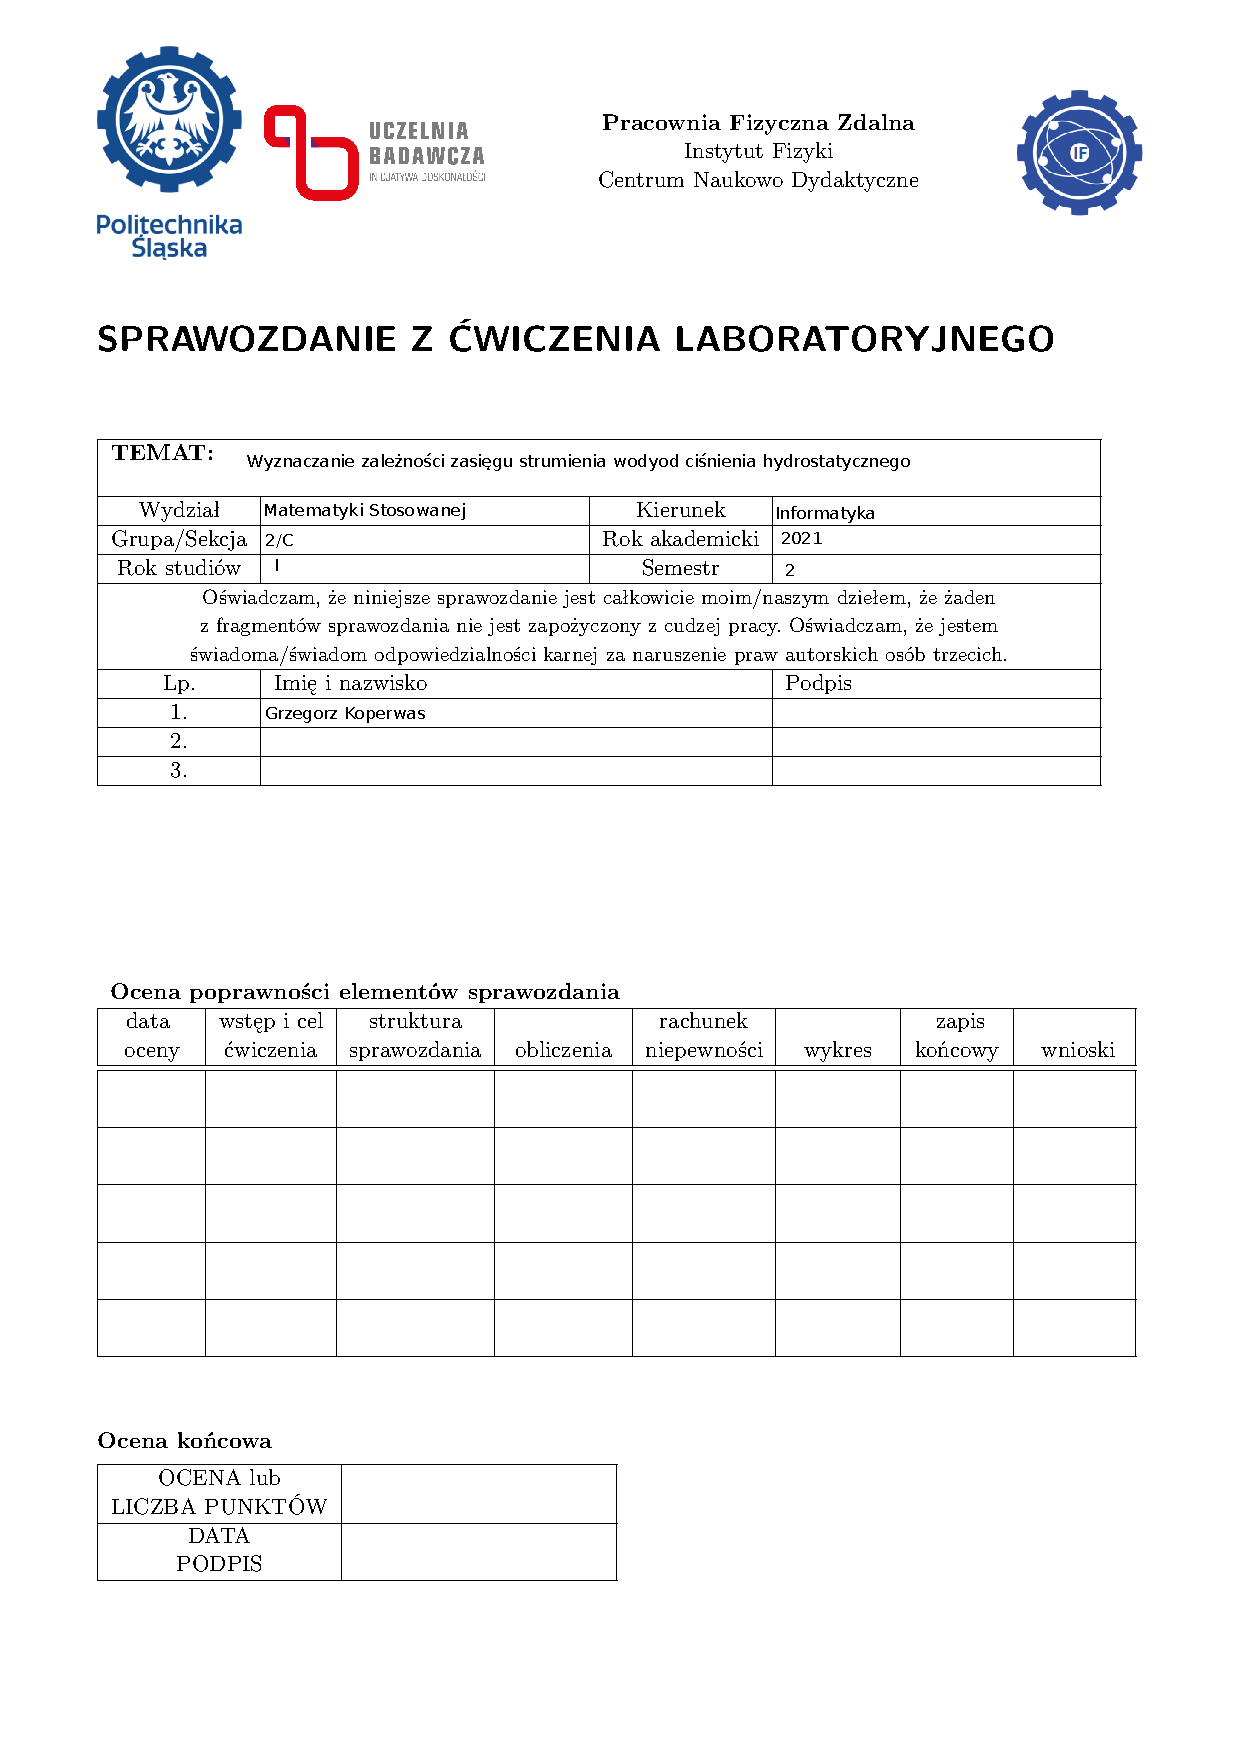
\includepdf[pages=-]{PFZ-StrTytulowa.pdf}

\section{Wstęp teoretyczny}

Celem doświadczenia jest zbadanie zależności między zasięgiem strumienia wody $z$ a ciśnieniem hydrostatycznym w naczyniu, oraz wyznaczenie prędkości wypływającej cieczy w zależności od ciśnienia.

\begin{figure}[h]
	\begin{tikzpicture}
		\fill [pattern = north east lines, pattern color=blue, draw=none, fill] (0, 0) rectangle (3, 3);
		\draw [thick] (0, 3.1) -- (0, 1.05);
		\draw [thick] (0, .95) -- (0, 0) -- (3, 0) -- (3, 3.1);
		\draw [thin, dashed] (0, 1) -- (3.5, 1);
		\draw [thin, dashed] (3, 3) -- (3.5, 3);
		\draw [thin, dashed] (3, 0) -- (3.5, 0);
		\draw [<->] (3.5, 1) -- (3.5, 3) node[pos=.5, right] {$h$};
		\draw [<->] (3.5, 0) -- (3.5, 1) node[pos=.5, right] {$H$};
		\draw [->, thin] (0, 1) -- (-1, 1) node[left] {$\vec{v}$};
		\draw [color=blue, thick] (-2, 0) arc [start angle=180, end angle=90, x radius=2, y radius=1];
		\draw [<->] (-2, 0) -- (0, 0) node[pos=.5, below] {$z$};
	\end{tikzpicture}
	\centering
	\caption{Układ pomiarowy}\label{rys:układ}
\end{figure}

\subsection*{Ciśnienie a zasięg}

Ciśnienie hydrostatyczne w układnie na rysunku \ref{rys:układ} jest dane wzorem:
\[ P = \rho g h\]

Gdzie $h$ jest mierzone bezpośrednio poprzez podziałkę na pojemniku (butelce), a $\rho$ jest ustalane za pomocą wartości tablicowych w zależności od temperatury otoczenia.

\subsection*{Wyznaczenie prędkości wypływającej cieczy}

Zasięg rzutu poziomego jest dany wzorem:
\[z = v \sqrt{\frac{2 H}{g}}\]

Zatem prędkość wypływającej cieczy jest dana wzorem:

\[v = z \sqrt{\frac{g}{2 H}}\]

Z równania \emph{Bernouliego} wynika że:
\begin{align*}
	\rho g h + p_1                                   & = p_2 + \frac{\rho v^2}{2}          \\
	\left(gh + \frac{p_1 - p_2}{\rho}\right) \cdot 2 & = v^2,\quad \text{Niech } p_1 = p_2 \\
	\sqrt{2gh}                                       & = v
\end{align*}

Zatem powinna zachodzić zależność:
\begin{equation*}
	z \sqrt{\frac{1}{2H}} = \sqrt{2h}\qquad \left| \cdot \sqrt{2H} \right. 
\end{equation*}
\begin{equation}
	z = 2\sqrt{hH}
\end{equation}\label{eq:should}

\section{Wyniki pomiarów:}

Na podstawie danych z tablicy \ref{tab:stale} odczytujemy że $\rho = 997,91 \frac{kg}{m^3}$

\begin{table}[hbt]
	\centering
	\begin{tabular}{|l|l|l|r|}
		\hline
		\multirow{2}{*}{\begin{tabular}[c]{@{}l@{}}$h$ [cm]\\ $\pm 0,2cm$\end{tabular}} & \multicolumn{3}{l|}{Zasięg $z$ [cm] $\pm 0,2cm$}             \\ \cline{2-4}
		                                           & 1.                                               & 2.  & 3.  \\ \hline\hline
		6,0                                        & 6,5                                              & 6,5 & 6,2 \\ \hline
		5,0                                        & 6,0                                              & 5,5 & 5,3 \\ \hline
		4,5                                        & 5,0                                              & 4,2 & 4,5 \\ \hline
		4,0                                        & 4,0                                              & 3,6 & 3,6 \\ \hline
		3,5                                        & 3,5                                              & 3,0 & 2,5 \\ \hline
	\end{tabular}
	\caption{Wyniki pomiarów}\label{tab:raw}
\end{table}

\begin{figure}[hbt]
	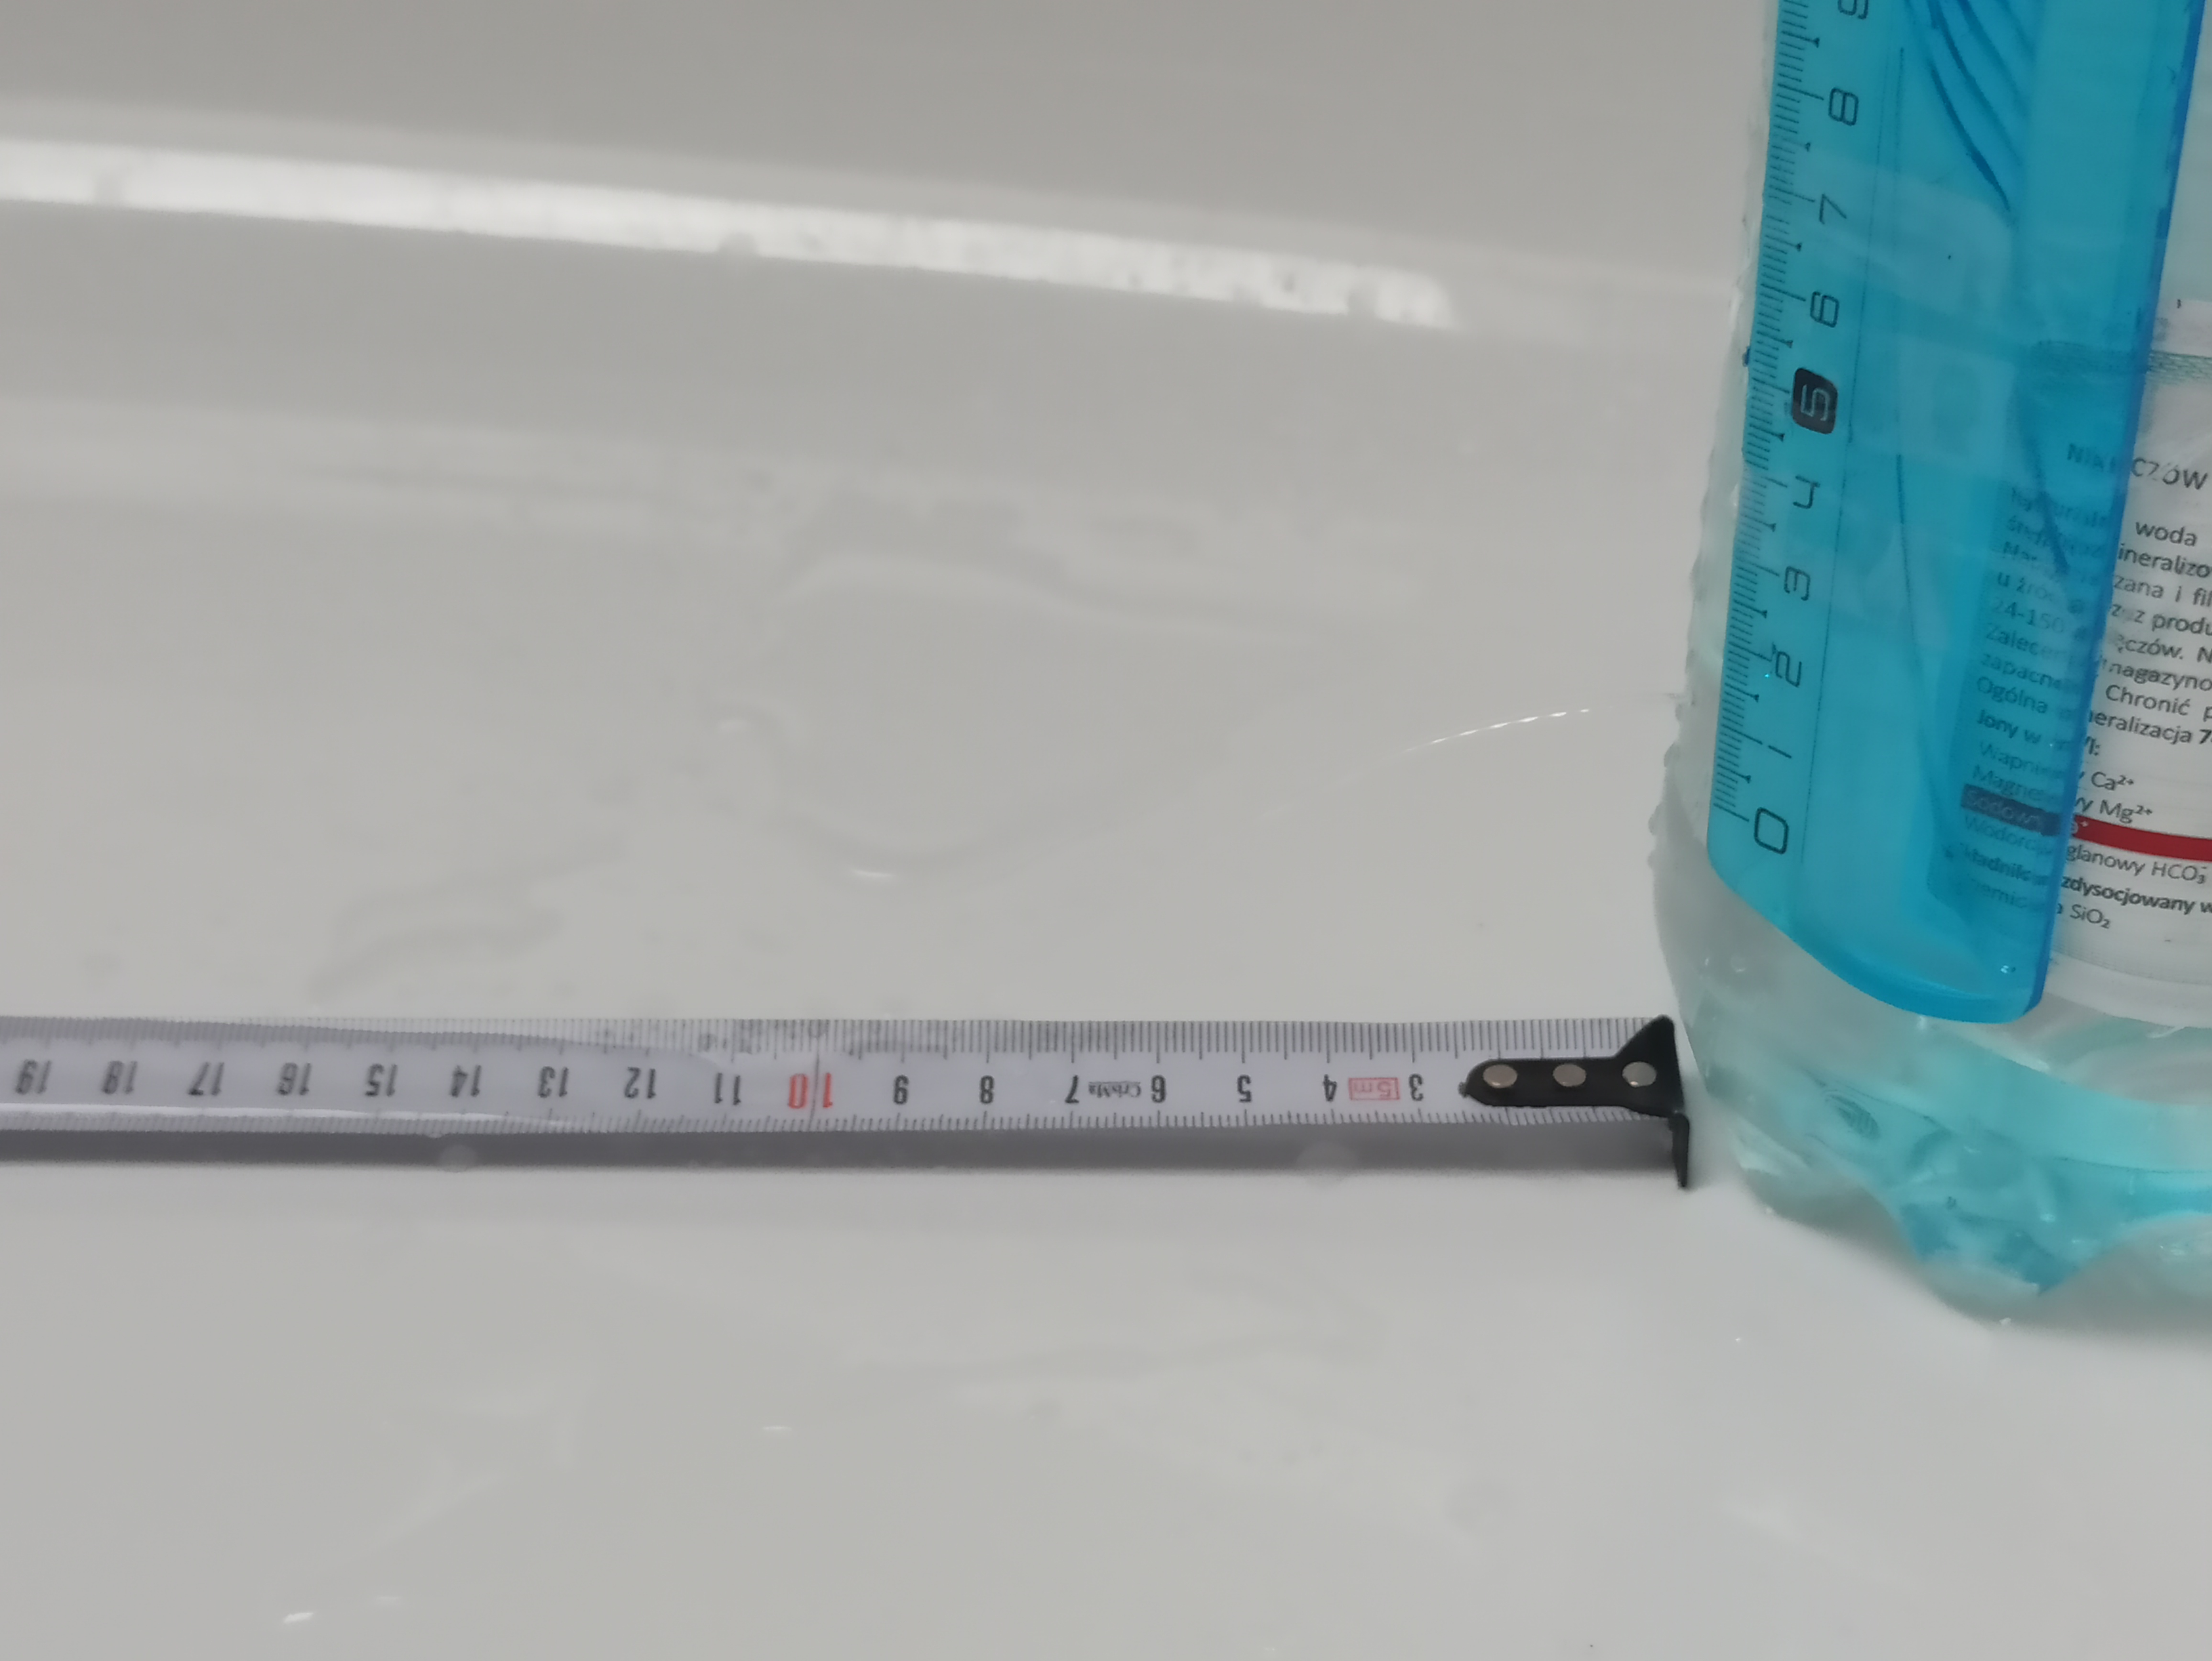
\includegraphics[scale=.05]{stanowisko.jpg}
	\centering
	\caption{Stanowisko pomiarowe}
\end{figure}

\begin{table}[hbt]
\centering
\begin{tabular}{|l|l|}
\hline
Stała                                 & Wartość \\ \hline\hline
T [$\stopnie C$] $\pm 0,5 \stopnie C$ & 21,5    \\ \hline
H [cm] $\pm 0,2cm$                    & 6,0     \\ \hline
\end{tabular}
\caption{Inne wartości}
\label{tab:stale}
\end{table}

\clearpage

\section{Przetwarzanie danych oraz obliczone wartości}

\subsection*{Zależność zasięgu od ciśnienia}

\begin{table}[h]
\centering
\begin{tabular}{|l|l|l|l|l|l|l|l|}
\hline
\begin{tabular}[c]{@{}l@{}}$h$ [cm]\\ $\pm 0,2cm$\end{tabular} &
  $\bar{z}$ [cm] &
  $u\left(\bar{z}\right)$ &
  $u\left(z_{cal}\right)$ &
  $P$ [Pa] &
  $u\left( P \right)$ &
  $z^2$ [$cm^2$] &
  $u\left( z^2 \right)$ \\ \hline\hline
6,0 & 6,4 & 0,13 & 0,24 & 587,37 & 19,58 & 41,0 & 0,48 \\ \hline
5,0 & 5,6 & 0,27 & 0,34 & 489,47 & 19,58 & 31,4 & 0,68 \\ \hline
4,5 & 4,6 & 0,31 & 0,37 & 440,53 & 19,58 & 20,9 & 0,73 \\ \hline
4,0 & 3,7 & 0,18 & 0,27 & 391,58 & 19,58 & 13,9 & 0,53 \\ \hline
3,5 & 3,0 & 0,38 & 0,43 & 342,63 & 19,58 & 9,0  & 0,86 \\ \hline
\end{tabular}
\caption{Przetworzone wartości}\label{tab:processed}
\end{table}
\begin{figure}[h]
	\input{PfromZ2.pgf}
	\centering
	\caption{Wykres $P$ od $z^2$}\label{rys:wykres1}
\end{figure}

\subsection*{Wyznaczanie prędkości wypływu cieczy}

\section{Wnioski}
\section{Sposoby na ograniczenie błędów}
\end{document}
